
%使用XeLaTeX编译
%版权所有,翻版必究
%本文件由程序自动生成,任何修改将被覆盖
%2019 年 01 月 23 日




\FloatBarrier
\section{
在Qt Quick中使用着色器
}\label{s100610}


%begin图片
\begin{figure}[htb] %浮动体 here and top ...
%there must use marginnote ...
\marginnote{\setlength\fboxsep{2pt}\fbox{\footnotesize{\kaishu\figurename\,}\footnotesize{\ref{p000008}}}}\centering %中心对齐
\setlength\fboxsep{-1pt}\fbox{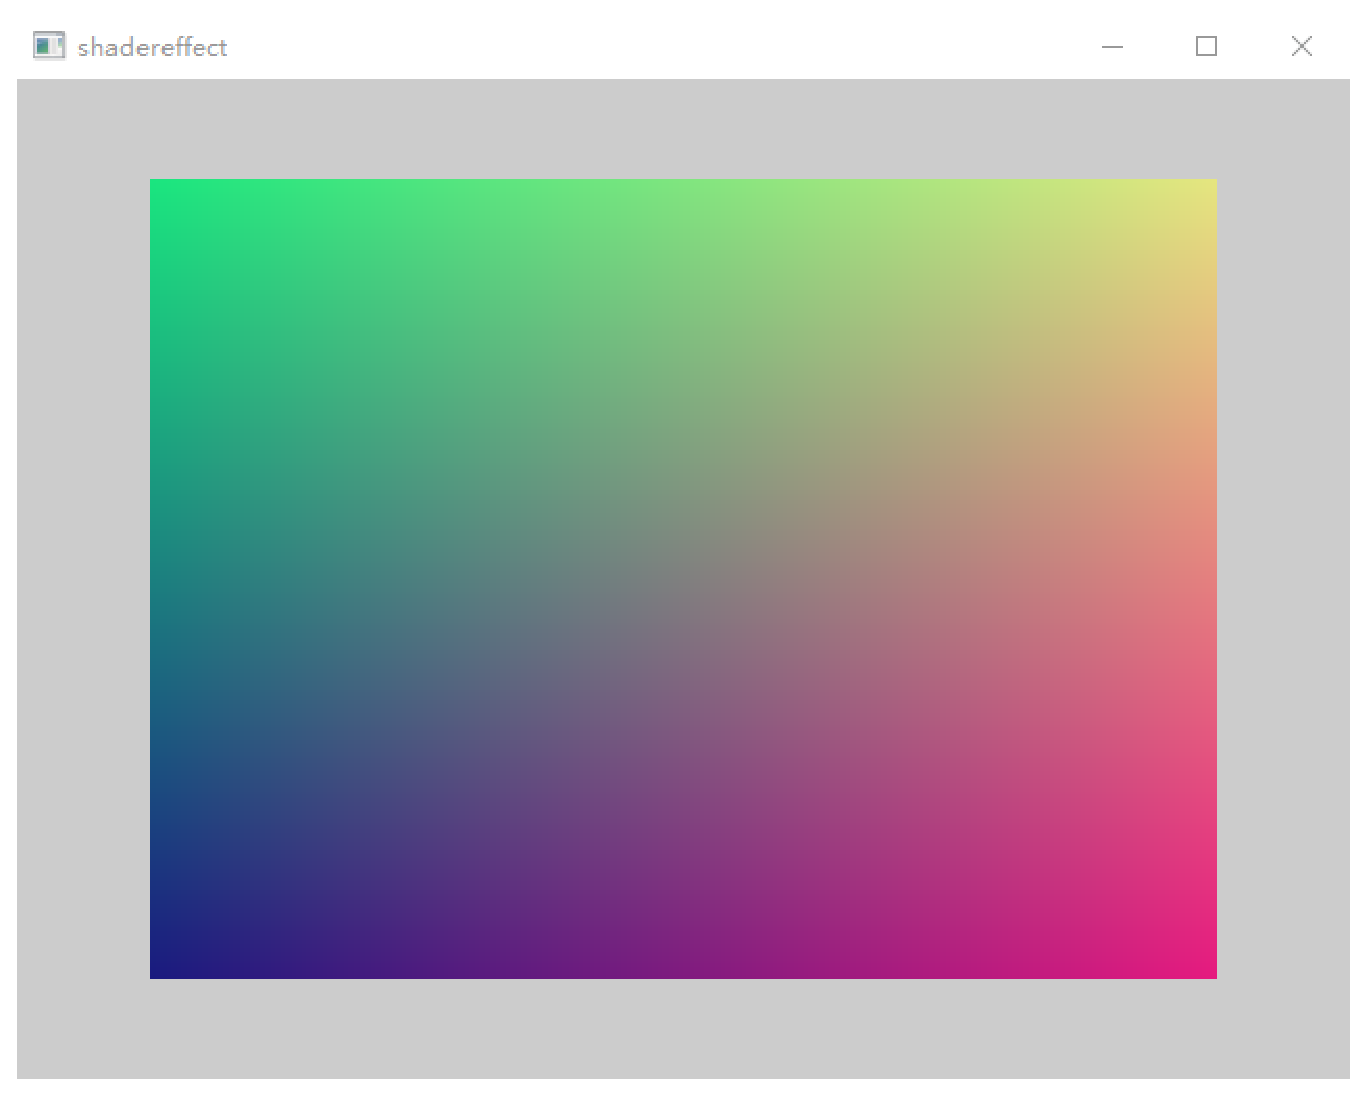
\includegraphics[width=0.95\textwidth]{the_book_image/p000008.eps}} %图片路径
\caption{Qt Quick中使用着色器} %标题
\label{p000008} %索引
\end{figure}
%end图片


Qt Quick本身是使用OpenGL达成渲染的,
Qt Quick原生支持GLSL。

不过,考虑到硬件兼容性。目前在Qml中
使用GLSL,只支持
顶点着色器和片段着色器。

如果读者需要使用计算着色器、几何着色器或分型着色器,
读者需要使用C{\sourcefonttwo{}+}{\sourcefonttwo{}+}扩展Qml。

如\filesourcenumbernameone\ \ref{f000038}
第14\raisebox{0.16ex}{\sourcefonttwo\~{}}46行展示了如何使用“ShaderEffect”,在
Qt Quick中使用GLSL。

%\begin{spacing}{1.0}
\refstepcounter{filesourcenumber}\label{f000038}    %增加源代码编号
\FloatBarrier                                  %强制完成浮动体布局
\begin{thebookfilesourceone}[escapeinside={(*@}{@*)},
caption=GoodLuck,
title=\filesourcenumbernameone \thefilesourcenumber
]
/*shadereffect/main.qml*/
import QtQuick 2.9

Rectangle {

    width: 640;
    height: 480;
    color: Qt.rgba(0.8,0.8,0.8,1);

    Rectangle{
        anchors.centerIn: parent    ;
        width: parent.width * 0.8   ;
        height: parent.height * 0.8 ;
        ShaderEffect{
            anchors.fill: parent ;
            fragmentShader:"
/*片段着色器*/
#version 460

in vec2  qt_TexCoord0/*纹理坐标*/  ;
out vec4 fragColor   /*输出值*/    ;

uniform float qt_Opacity/*透明度*/ ;

void main() {
    vec4 varColor  = vec4( qt_TexCoord0.x ,  qt_TexCoord0.y , 0.5 , 1);
    fragColor = varColor * qt_Opacity;
}

"
            vertexShader :"
/*顶点着色器*/
#version 460

in vec4 qt_Vertex/*输入点坐标*/    ;
out vec2 qt_TexCoord0/*纹理坐标*/  ;

uniform mat4 qt_Matrix/*投影矩阵*/ ;

void main() {
    gl_Position = qt_Matrix * qt_Vertex;
    qt_TexCoord0 = gl_Position.xy*0.5 + 0.5 ;
}

"
        }
    }

}/*~Rectangle*/(*@\marginpar[\hfill\setlength\fboxsep{2pt}\fbox{\footnotesize{\kaishu\parbox{1em}{\setlength{\baselineskip}{2pt}\filesourcenumbernameone}}\footnotesize{\thefilesourcenumber}}]{\setlength\fboxsep{2pt}\fbox{\footnotesize{\kaishu\parbox{1em}{\setlength{\baselineskip}{2pt}\filesourcenumbernameone}}\footnotesize{\thefilesourcenumber}}}@*)\end{thebookfilesourceone}          %抄录环境
\addtocounter{lstlisting}{-1}   %sub lstlisting counter ...
%\end{spacing}
%main.qml

%%%%%%%%%%%%%%%%%%%%%%%%%%%%%%%%%%

使用“ShaderEffect”导入纹理是极为简单的。
读者只需要在“ShaderEffect”自定义
一个代表“Image”的属性,
在GLSL中就可以直接使用了。

如\filesourcenumbernameone\ \ref{f000039}
所示:

\begin{itemize}

\item 第14\raisebox{0.16ex}{\sourcefonttwo\~{}}18行定义了一个Image;
\item 第20行定在“ShaderEffect”中自定义了
一个名为的“source”属性,此属性指向Image对象;
\item 第30行在片段着色器中将
“source”属性作为一个纹理载入;

\end{itemize}

%begin图片
\begin{figure}[htb] %浮动体 here and top ...
%there must use marginnote ...
\marginnote{\setlength\fboxsep{2pt}\fbox{\footnotesize{\kaishu\figurename\,}\footnotesize{\ref{p000009}}}}\centering %中心对齐
\setlength\fboxsep{-1pt}\fbox{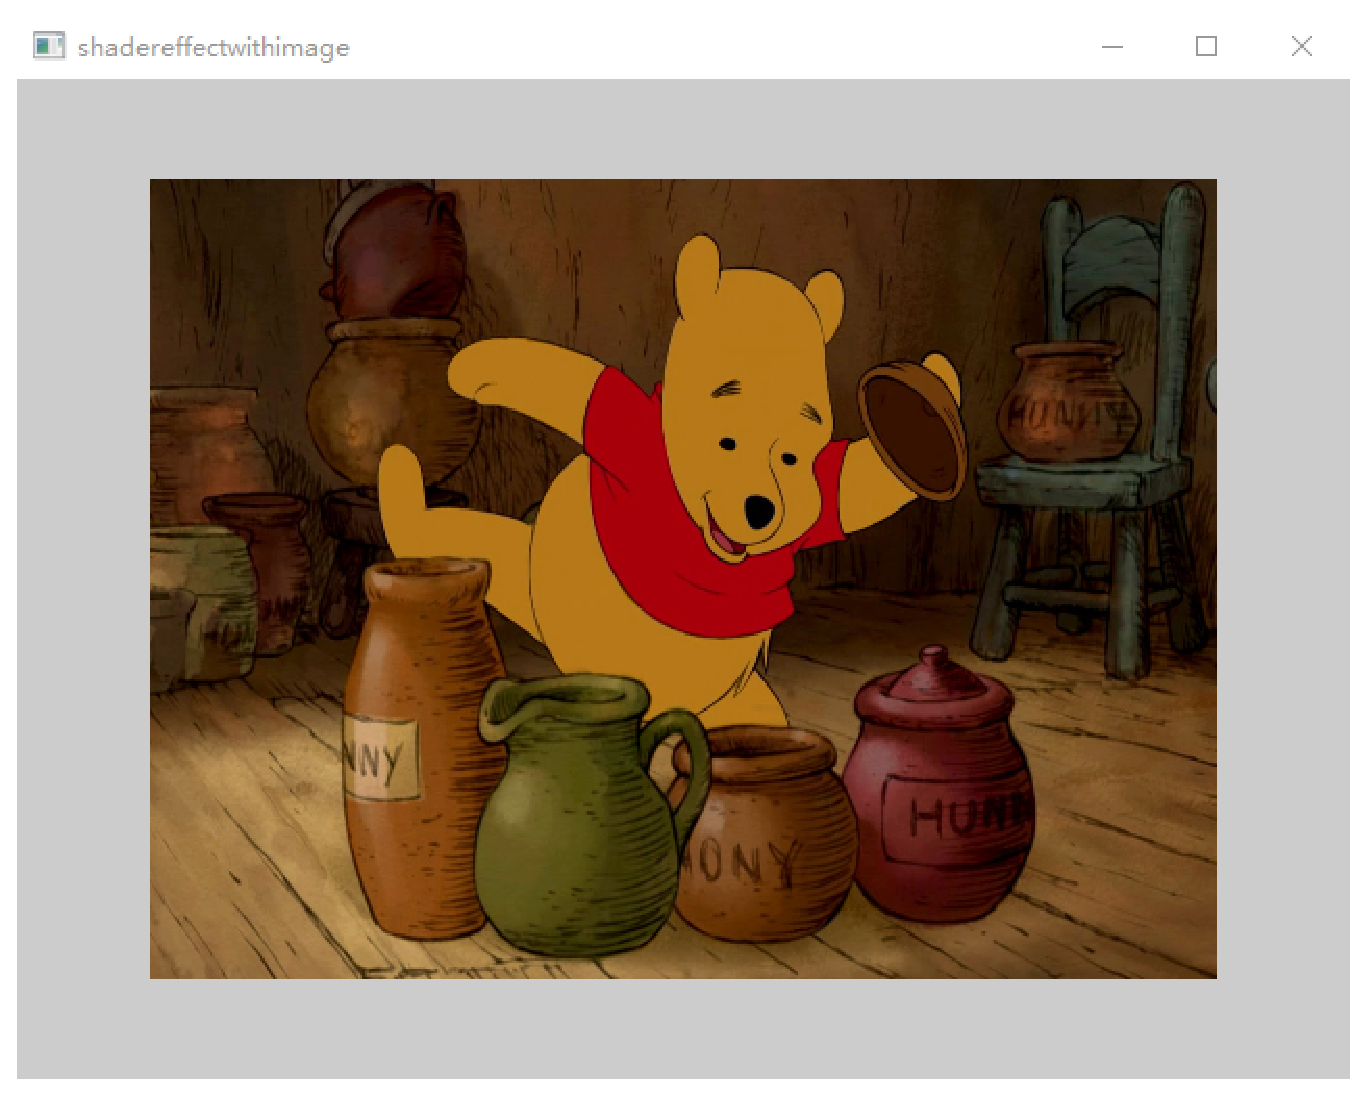
\includegraphics[width=0.95\textwidth]{the_book_image/p000009.eps}} %图片路径
\caption{Qt Quick着色器中使用纹理} %标题
\label{p000009} %索引
\end{figure}
%end图片


%\begin{spacing}{1.0}
\refstepcounter{filesourcenumber}\label{f000039}    %增加源代码编号
\FloatBarrier                                  %强制完成浮动体布局
\begin{thebookfilesourceone}[escapeinside={(*@}{@*)},
caption=GoodLuck,
title=\filesourcenumbernameone \thefilesourcenumber
]
/*shadereffectwithimage/main.qml*/
import QtQuick 2.9

Rectangle {

    width: 640;
    height: 480;
    color: Qt.rgba(0.8,0.8,0.8,1);

    Rectangle{
        anchors.centerIn: parent    ;
        width: parent.width * 0.8   ;
        height: parent.height * 0.8 ;
        Image{
            id : idSourceImage;
            source: "0000.jpg";
            visible: false    ;
        }
        ShaderEffect{
            property variant source: idSourceImage/*the image...*/
            anchors.fill: parent ;
            fragmentShader:"
/*片段着色器*/
#version 460

in vec2 qt_TexCoord0;

out vec4 fragColor;

uniform sampler2D source/*the image...*/;
uniform float qt_Opacity;

void main() {
    fragColor = texture(source, qt_TexCoord0) * qt_Opacity;
}

"
            vertexShader :"
/*顶点着色器*/
#version 460

in vec4 qt_Vertex;
in vec2 qt_MultiTexCoord0;

out vec2 qt_TexCoord0;

uniform mat4 qt_Matrix;

void main() {
    qt_TexCoord0 = qt_MultiTexCoord0;
    gl_Position = qt_Matrix * qt_Vertex;
}

"
        }
    }

}/*~Rectangle*/(*@\marginpar[\hfill\setlength\fboxsep{2pt}\fbox{\footnotesize{\kaishu\parbox{1em}{\setlength{\baselineskip}{2pt}\filesourcenumbernameone}}\footnotesize{\thefilesourcenumber}}]{\setlength\fboxsep{2pt}\fbox{\footnotesize{\kaishu\parbox{1em}{\setlength{\baselineskip}{2pt}\filesourcenumbernameone}}\footnotesize{\thefilesourcenumber}}}@*)\end{thebookfilesourceone}          %抄录环境
\addtocounter{lstlisting}{-1}   %sub lstlisting counter ...
%\end{spacing}
%main.qml


























%使用XeLaTeX编译
%版权所有,翻版必究
%本文件由程序自动生成,任何修改将被覆盖
%2019 年 01 月 23 日



